\documentclass{assignment}

\usepackage{fancyvrb}
\usepackage{url}

\mytitle{C4M: Dijkstra’s Shortest Path Worksheet}

\begin{document}

Consider the contents of file \verb|cities.txt| below, which represents data about a flight network shown in the picture on the right:

\vspace*{-0.3cm}
\begin{minipage}[c]{0.45\linewidth}
\begin{verbatim}
  Toronto:New York 3
  New York:Washington 2
  Washington:San Francisco 3
  San Francisco:Mexico City 3
  Toronto:Mexico City 7
  Toronto:San Francisco 6
\end{verbatim}
\end{minipage}
\hspace{1cm}
\begin{minipage}[c]{0.45\linewidth}
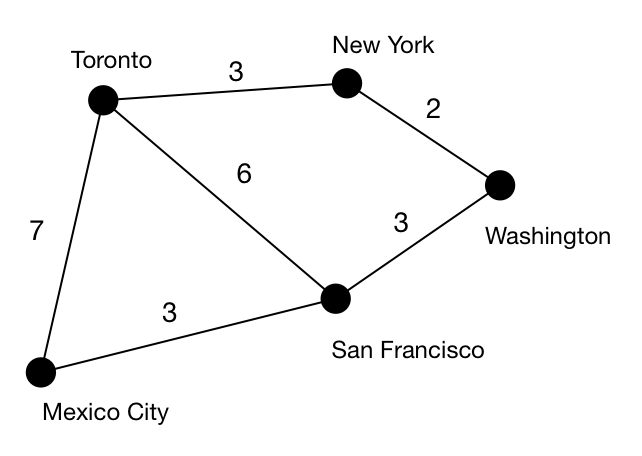
\includegraphics[width=6cm]{figs/map.png}
\end{minipage}

\vspace*{-0.6cm}\subsection*{Dijkstra's Shortest Path Algorithm}

Trace Dijkstra's shortest path algorithm on paper (writing down the visited and unvisited lists) using the example data above to find the shortest path from Toronto to every other city. \\

\texttt{unvisited = [('Toronto', 0)]}\\
\texttt{visited = []}
\end{document}
